\section{Consuntivo di periodo}

Di seguito vengono indicate le spese effettivamente sostenute per ogni ruolo, confrontate con quanto preventivato. Il bilancio potrà risultare:

\begin{itemize}
\item \textbf{positivo:} se il consuntivo è minore di quanto preventivato;
\item \textbf{pari:} se il consuntivo è uguale a quanto preventivato;
\item \textbf{negativo:} se il consuntivo è maggiore di quanto preventivato.
\end{itemize}

\subsection{Fase di analisi}
\subsubsection{Prospetto orario}
In questa fase, la distribuzione oraria dei componenti del gruppo è la seguente:

{

\rowcolors{2}{azzurro2}{azzurro3}

\centering
\renewcommand{\arraystretch}{1.8}
\begin{longtable}{C{4cm} C{1cm} C{1cm} C{1cm} C{1cm} C{1cm} C{1cm} C{2cm}}

\rowcolor{azzurro1}
\textbf{Nominativo} &
\textbf{RE}&
\textbf{AM}&
\textbf{AN}&
\textbf{PT}&
\textbf{PR}&
\textbf{VE}&
\textbf{Ore totali}\\
\endhead

\MB & 15 & 0 & 12 & 0 & 0 & 8 & 35 \\
\VAS & 0 & 18 & 5 & 0 & 0 & 12 & 35 \\
\FD & 10 & 8 & 5 & 0 & 0 & 12 & 35 \\
\NM & 0 & 20 & 5 & 0 & 0 & 10 & 35 \\
\SB & 0 & 18 & 7 & 0 & 0 & 10 & 35 \\
\GB & 0 & 0 & 22 & 0 & 0 & 13 & 35 \\
\MDI & 0 & 0 & 24 & 0 & 0 & 11 & 35 \\
\textbf{Ore Totali} & 25 & 64 & 80 & 0 & 0 & 76 & 245 \\

\rowcolor{white}
\caption{Distribuzione oraria nel periodo di analisi}\\

\end{longtable}
}
\newpage
Il seguente istogramma riassume i dati ottenuti:

\begin{figure}[H]
\centering
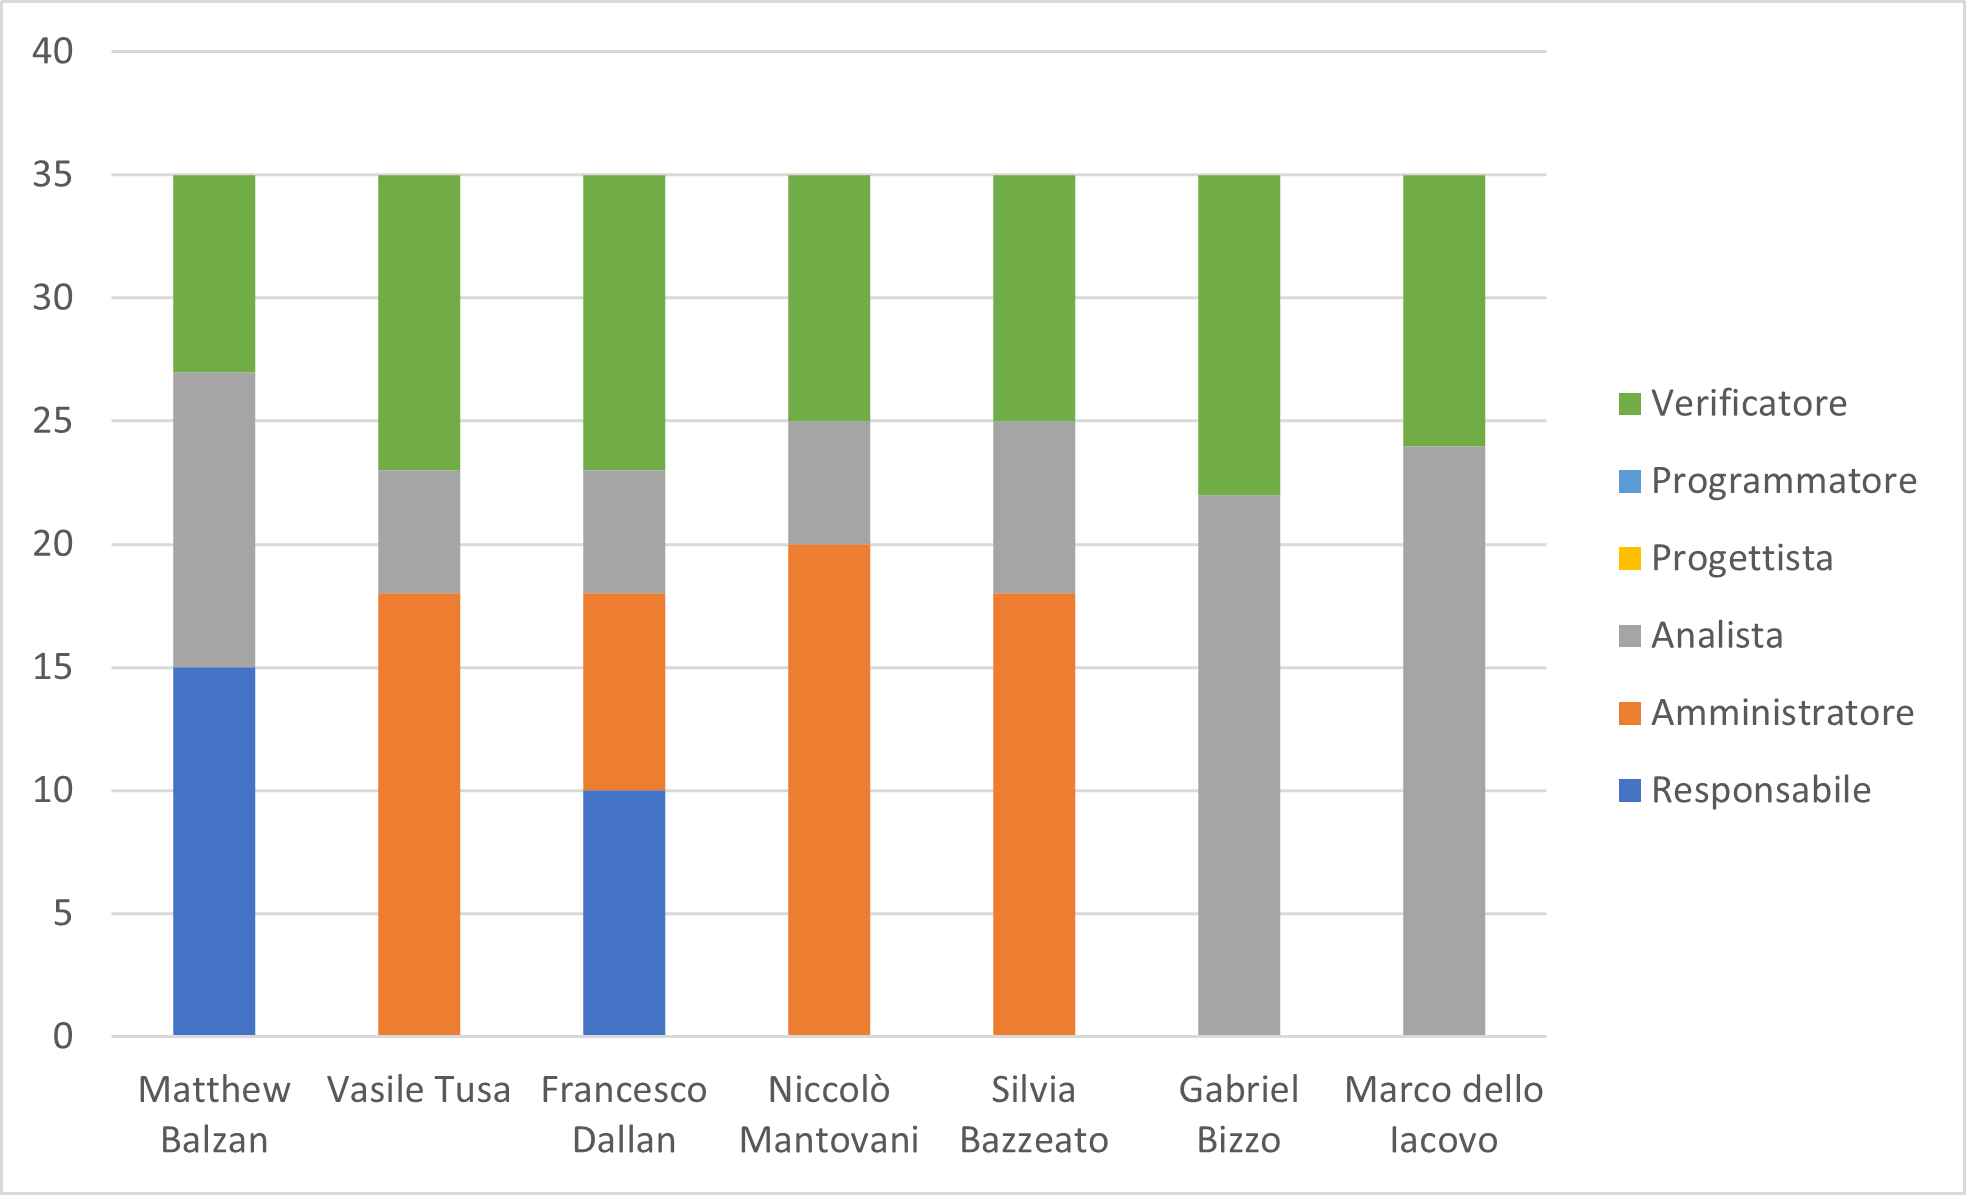
\includegraphics[scale=0.90]{res/Preventivo/Img/istogramma_analisi}\\
\caption{Istogramma della ripartizione dei ruoli nel periodo di analisi}
\end{figure}


\subsubsection{Prospetto economico}

In questa fase, il costo per ogni ruolo è il seguente:

{

\rowcolors{2}{azzurro2}{azzurro3}

\centering
\renewcommand{\arraystretch}{1.8}
\begin{longtable}{C{3cm} C{1cm} C{2cm} }

\rowcolor{azzurro1}
\textbf{Ruolo} &
\textbf{Ore}&
\textbf{Costo}\\
\endhead

\textit{Responsabile} & 25 & 750\euro{} \\
\ammProg & 64 & 1280\euro{} \\
\analProg & 80 & 2000\euro{} \\
\progetProg & 0 & 0\euro{} \\
\programProg & 0 & 0\euro{} \\
\verifProg & 76 & 1140\euro{} \\
\textbf{Totale} & 245 & 5170\euro{} \\

\rowcolor{white}
\caption{Prospetto dei costi per ruolo nel periodo di analisi}\\

\end{longtable}
}
\newpage
Il seguente areogramma riassume i dati ottenuti:

\begin{figure}[H]
\centering
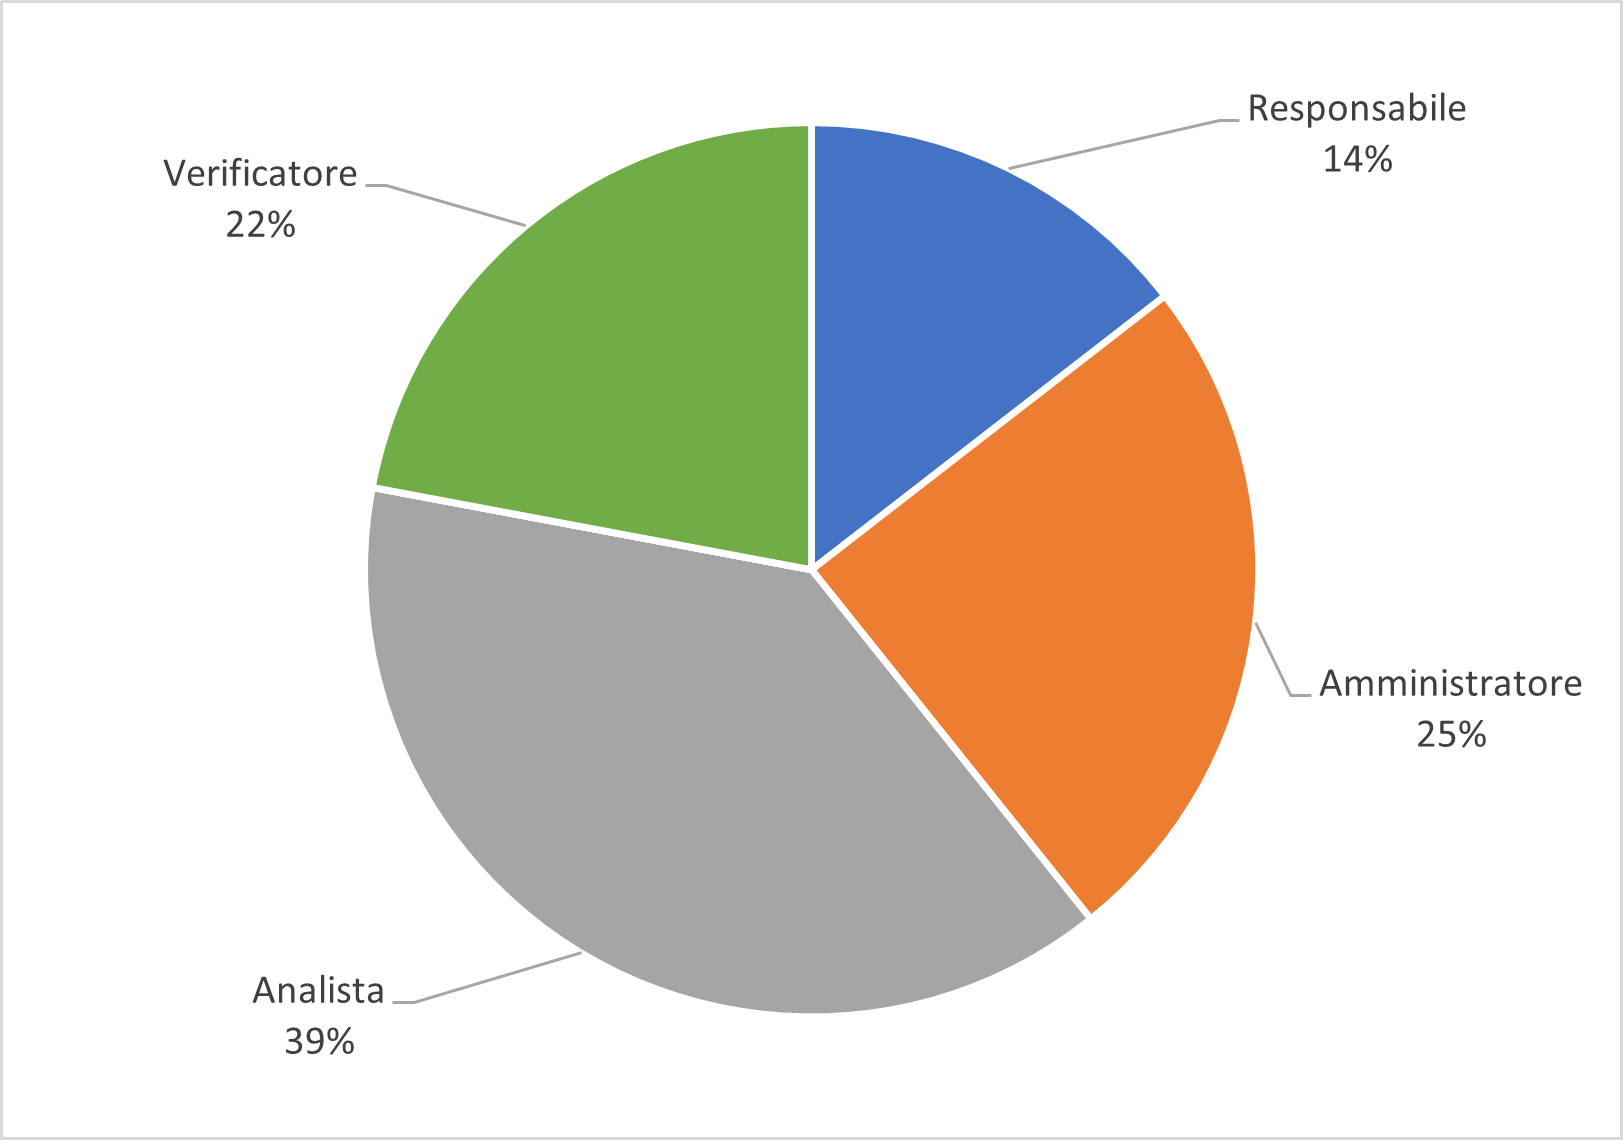
\includegraphics[scale=0.90]{res/Preventivo/Img/areogramma_analisi}\\
\caption{Areogramma della distribuzione economica nel periodo di analisi}
\end{figure}



